\documentclass[a4paper]{article}
\usepackage[utf8]{inputenc}
\usepackage[english,russian]{babel}
\usepackage{indentfirst}
\usepackage{misccorr}
\usepackage{graphicx}
\graphicspath{{pics/}}
\usepackage{amsmath}
\usepackage[nottoc,numbib]{tocbibind}
\usepackage{multicol}
\usepackage{float}
\DeclareMathOperator*{\argmin}{arg\,min}
\usepackage[a4paper,margin=1.5cm]{geometry}


\begin{document}

\begin{titlepage}
\thispagestyle{empty}

\begin{center}
\begin{figure}[htbp]
  \centering
  
\includegraphics[width=0.6\textwidth]{msu}
\end{figure}


Московский Государственный Университет им. М.В. Ломоносова

Факультет Вычислительной Математики и Кибернетики

Кафедра Автоматизации Систем Вычислительных Комплексов

\vfill
\textbf{\Huge Маршрутизация демультиплексированных соединений с учётом текущего состояния сети}

\vfill
{\huge Курсовая работа}
\end{center}

\vfill
\begin{flushright}
{\large Выполнил:\\Звонов Андрей Денисович\\321 группа\\}
\vspace{0.5cm}
{\large Научный руководитель:\\Степанов Евгений Павлович}
\end{flushright}

\vfill
\centerline{Москва, 2020 год}

\end{titlepage}
\linespread{1.5}
\setcounter{page}{2}
\large

\begin{abstract}
\large
В настоящей работе рассматривается задача нахождения множества оптимальных маршрутов в сети для демультиплексированного соединения. Использование многопоточных протоколов без эффективной политики маршрутизации подпотоков не даёт того выигрыша от демультиплексирования, который можно получить при её наличии.
Для этой задачи в данной работе предложены несколько алгоритмов её решения, проведено их экспериментальное исследование.

\end{abstract}
\newpage

\tableofcontents
\newpage

\section{Введение}

\subsection{Цель работы}
Целью данной работы является ускорение работы транспортных соединений при помощи использования алгоритма маршрутизации демультиплексированных соединений, учитывающего текущее состояние сети.\\
Под состоянием сети в данной работе будем понимать данные о доступной пропускной способности каждого канала в сети в некоторый момент времени. То, каким способом были получены эти данные, выходит за рамки данной работы.

\subsection{Актуальность}
Пусть необходимо передать через сеть упорядоченный поток байтов. Разобьём этот набор на несколько наборов, и каждый из этих наборов будем передавать отдельным транспортным соединением; такое соединение будем называть подпотоком. Демультиплексированное соединение --- соединение, в котором пересылаются данные в сети с использованием нескольких подпотоков одновременно.\\
В настоящее время широко используются многопоточные протоколы передачи данных, то есть протоколы, позволяющие работать с демультиплексированными соединениями \cite{mpusage}\cite{protos}. Демультиплексирование соединения позволяет увеличить его пропускную способность, так как используются пропускные способности не одного, а нескольких маршрутов в сети. Кроме того, демультиплексирование повышает и отказоустойчивость соединения. Напрмер, в случае отказа канала, через который проходит один из подпотоков, остальные не проходящие через этот канал подпотоки сохранят работоспособность.\\
Для работы с демультиплексированными соединениями существуют различные многопоточные протоколы, например, MultiPath TCP, или MPTCP\cite{mptcp}. Он позволяет разбить поток данных, получаемых от приложения, на несколько подпотоков и каждый из подпотоков передавать отдельным транспортным соединением. Причём MPTCP предоставляет приложению возможность работы с обычным TCP-сокетом, то есть приложение может не знать, что работает с MPTCP, и для передачи данных в сети также используются обычные TCP-соединения. При этом количество подпотоков статическое, то есть определяется до начала работы и в процессе работы не изменяется.\\
Протокол Flow (De) Multiplexing Protocol \cite{FDMP}, или FDMP, также разбивает поток  данных на несколько подпотоков; но, в отличие от MPTCP, количество используемых  подпотоков динамически изменяется во время работы в зависимости от требования к пропускной способности и состояния сети: в случае, если уже имеющиеся подпотоки не удовлетворяют требованию, происходит попытка открытия нового подпотока, а если при закрытии какого-либо подпотока оставшиеся смогут удовлетворить требованию, этот подпоток закрывается. \\Однако, ни один из этих алгоритмов не обеспечивает маршрутизацию установленного многопоточного соединения. Вместе с тем, использование многопоточных соединений без эффективных алгоритмов их маршрутизации может не дать того выигрыша от демультиплексирования, который можно было бы получить при её наличии.

\begin{figure}[H]
   \begin{minipage}{0.5\textwidth}
     \centering
     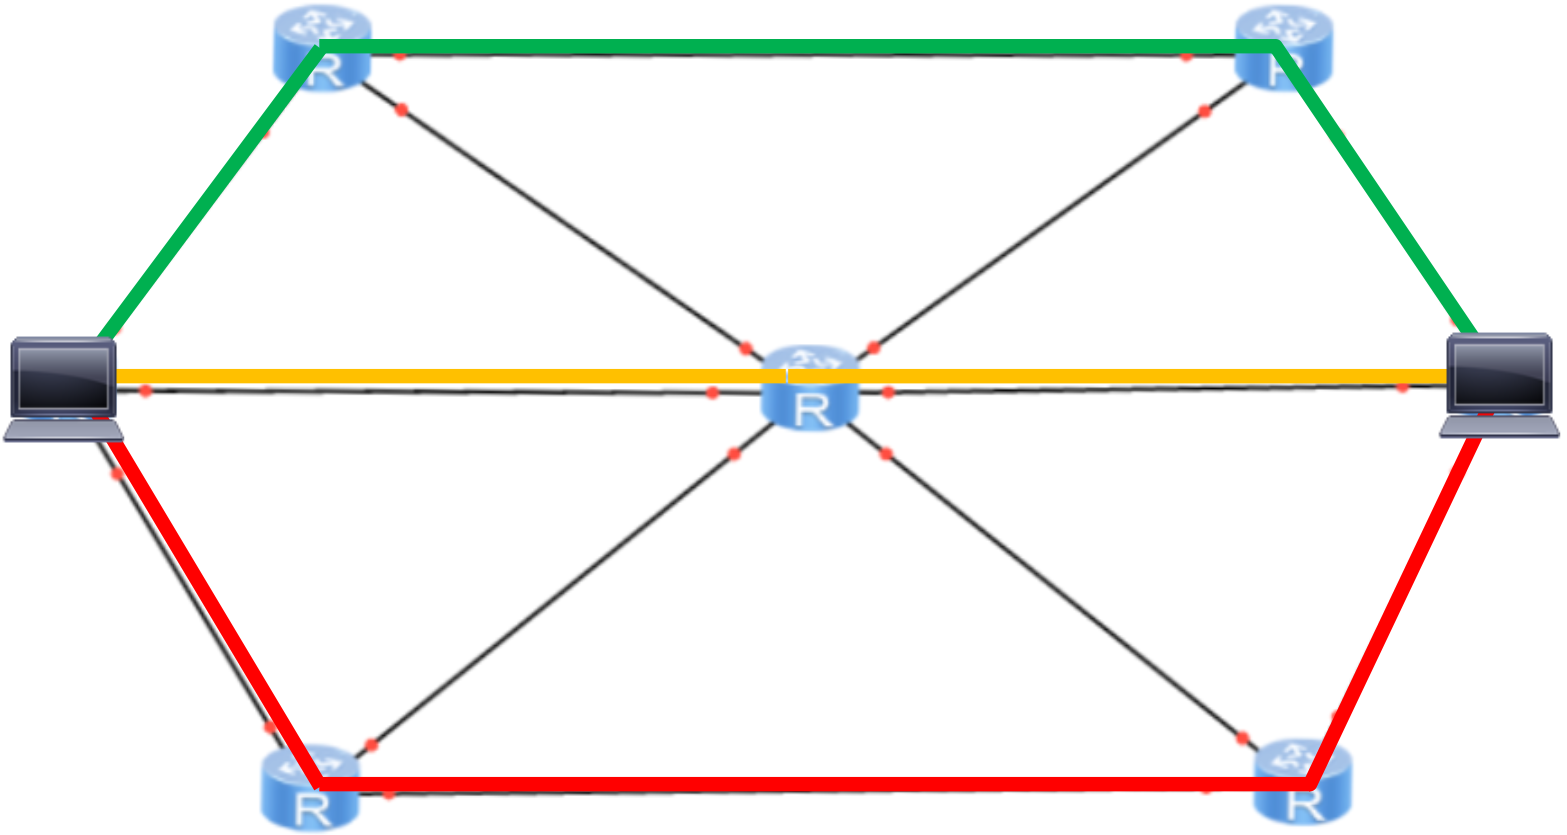
\includegraphics[width=.7\linewidth]{wrout.png}
     \caption{Пример маршрутов без пересечений}\label{Fig:Data1}
   \end{minipage}
   \begin{minipage}{0.5\textwidth}
     \centering
     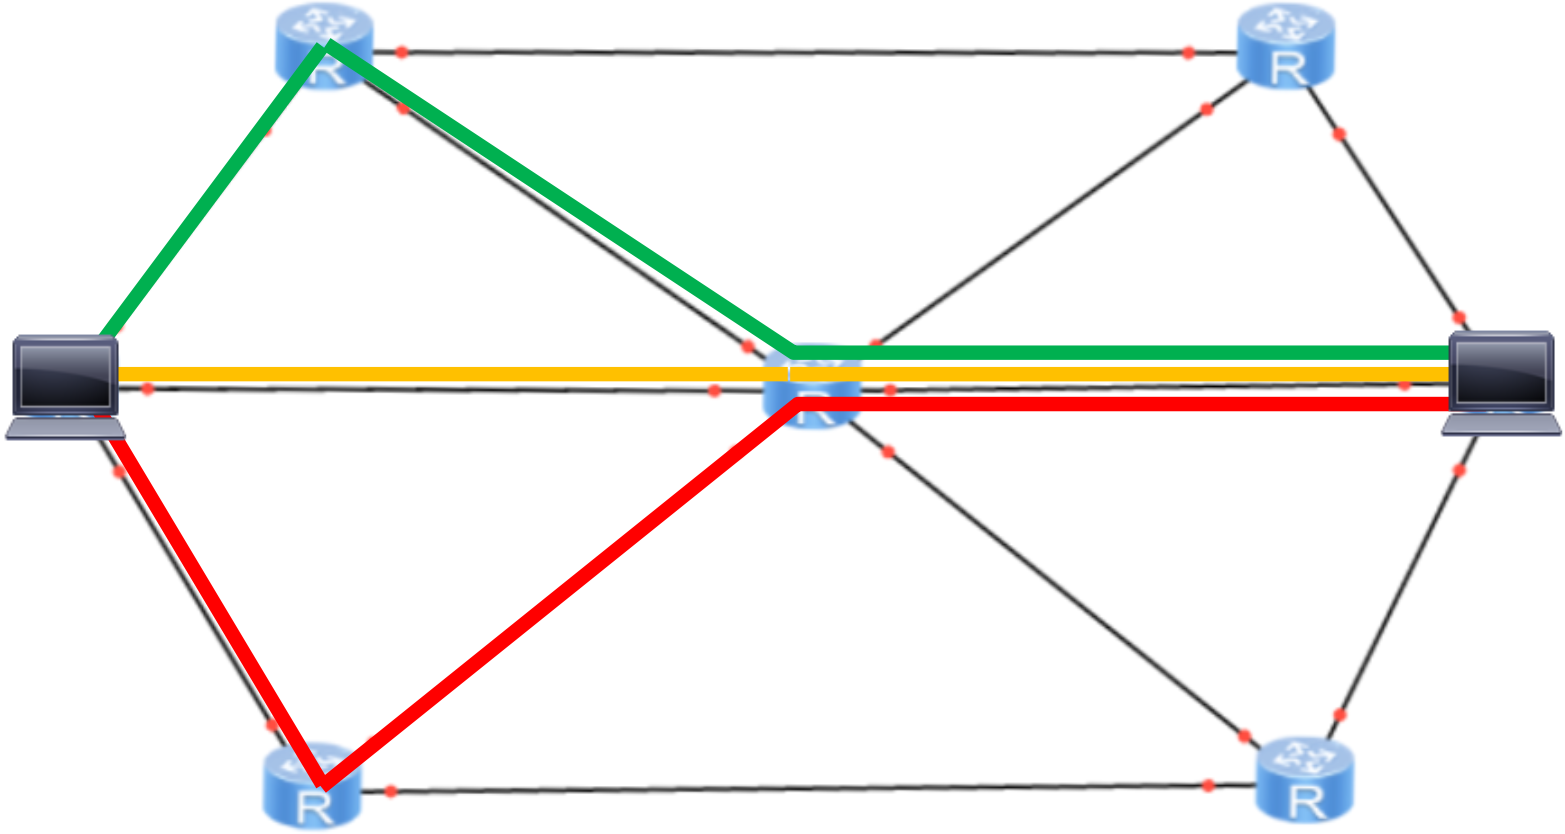
\includegraphics[width=.7\linewidth]{woutrout.png}
     \caption{Пример маршрутов с пересечениями}\label{Fig:Data2}
   \end{minipage}\hfill
\end{figure}

Пусть пропускная способность каждого канала в примере на рис. \ref{Fig:Data1} и \ref{Fig:Data2} равна 100 единиц. При выборе маршрутов как на рис. \ref{Fig:Data1} два абонента в этой сети смогут обмениматься данными со скоростью 300 единиц. Однако, при неправильном выборе множеста маршрутов (рис. \ref{Fig:Data2}), то есть имеющего большое количество пересечений по каналам между входящими в него маршрутами, может возникнуть узкое место, которое не даст получить того выигрыша от демультиплексирования, который был бы получен при правильном выборе маршрутов; в данном примере скорость передачи данных уже не превысит 100 единиц (что могло быть достигнуто и обыкновенным, не демультиплексированным, соединением). Кроме того, узкое место может появиться не сразу, а позже, при изменении состояния сети. Такое узкое место не только может уменьшить пропускную способность демультиплексированного соединения, но и уменьшает его отказоустойчивость --- в случае отказа канала, на котором пересекаются несколько подпотоков, все они утратят работоспособность.

В связи с этим возникает необходимость разработки алгоритма поиска множества маршрутов, удовлетворяющего заданному требованию к пропускной способности.

\subsection{Задачи работы}
Для достижения поставленной цели необходимо решить следующие задачи:
\begin{enumerate}
\item Провести обзор существующих алгоритмов поиска маршрутов для того, чтобы выбрать алгоритм, на основе которого будет предложено решение задачи выбора маршрутов для демультиплексированного соединения.
\item Разработать и реализовать алгоритм поиска маршрутов для демультиплексированных соединений, учитывающий текущее состояние сети.
\item Провести экспериментальное исследование прототипа разработанного алгоритма.
\end{enumerate}

\subsection{Структура работы}
Глава 2 содержит неформальную постановку задачи поиска множества маршрутов. В главе 3 приводится формальная постановка задачи. Глава 4 содержит обзор существующих алгоритмов, решающих схожие с поставленной задачи. В главе 5 описаны предложенные в рамках данной работы алгоритмы маршрутизации. В главе 6 представлены результаты экспериментального исследования этих алгоритмов.



\newpage
\section{Неформальная постановка задачи}
Пусть нам известно состояние сети в некоторый момент времени, которое представлено в виде ненаправленного графа без кратных рёбер, для каждого ребра задана его остаточная пропускная способность в некоторый момент времени. Кроме того, обозначены точка-отправитель и точка-получатель, и известно требование к пропускной способности.\\
До того, как ввести функцию стоимости маршрута и множества маршрутов, отметим, что данная задача как минимум принадлежит классу $NP-hard$ \cite{kmaxmin1}\cite{disjntNPC}, то есть нахождение не точного, а приближённого решения в данном случае оправдано.\\
Стоимость каждого маршрута будет зависеть от двух величин --- длины маршрута и избыточной занимаемой пропускной способности. 
Пусть изначально величина максимального потока в остаточном графе сети между выбранными вершинами была равна $mf_1$, а после выбора маршрута со скоростью, равной его максимальной пропускной способностью стала равна $mf_2$. Тогда, \textit{избыточной} занятой пропускной способностью назовём отношение разности $mf_1 - mf_2$ к максимальной пропускной способности рассматриваемого маршрута.\\
Стоимость же множества маршрутов будет складываться из индивидуальной стоимости всех входящих в него маршрутов и штрафа за каждое попарное пересечение по рёбрам между маршрутами множества.\\

\begin{figure}[!htb]
   \begin{minipage}{0.5\textwidth}
     \centering
     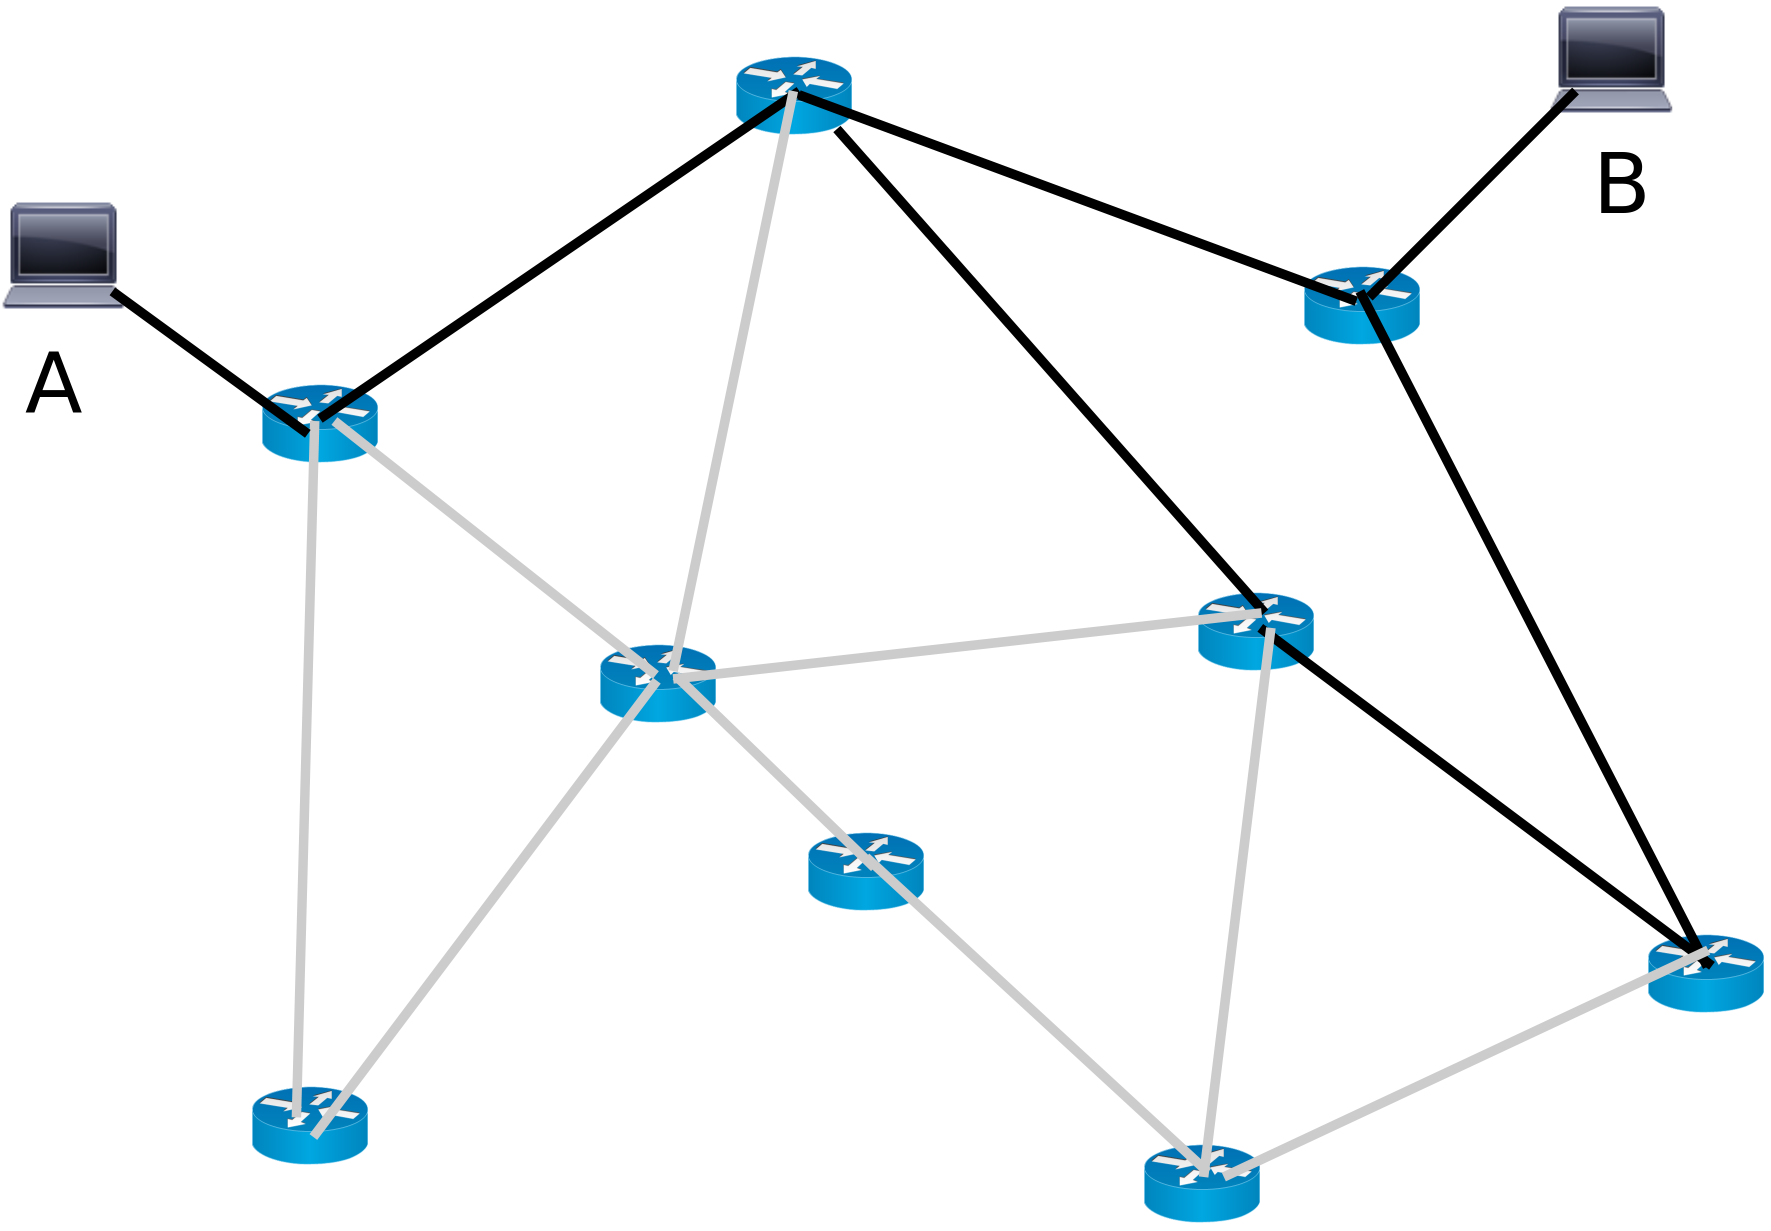
\includegraphics[width=.9\linewidth]{isect.png}
     \caption{Множество маршрутов с пересечениями}\label{Fig:Data3}
   \end{minipage}
   \begin{minipage}{0.5\textwidth}
     \centering
     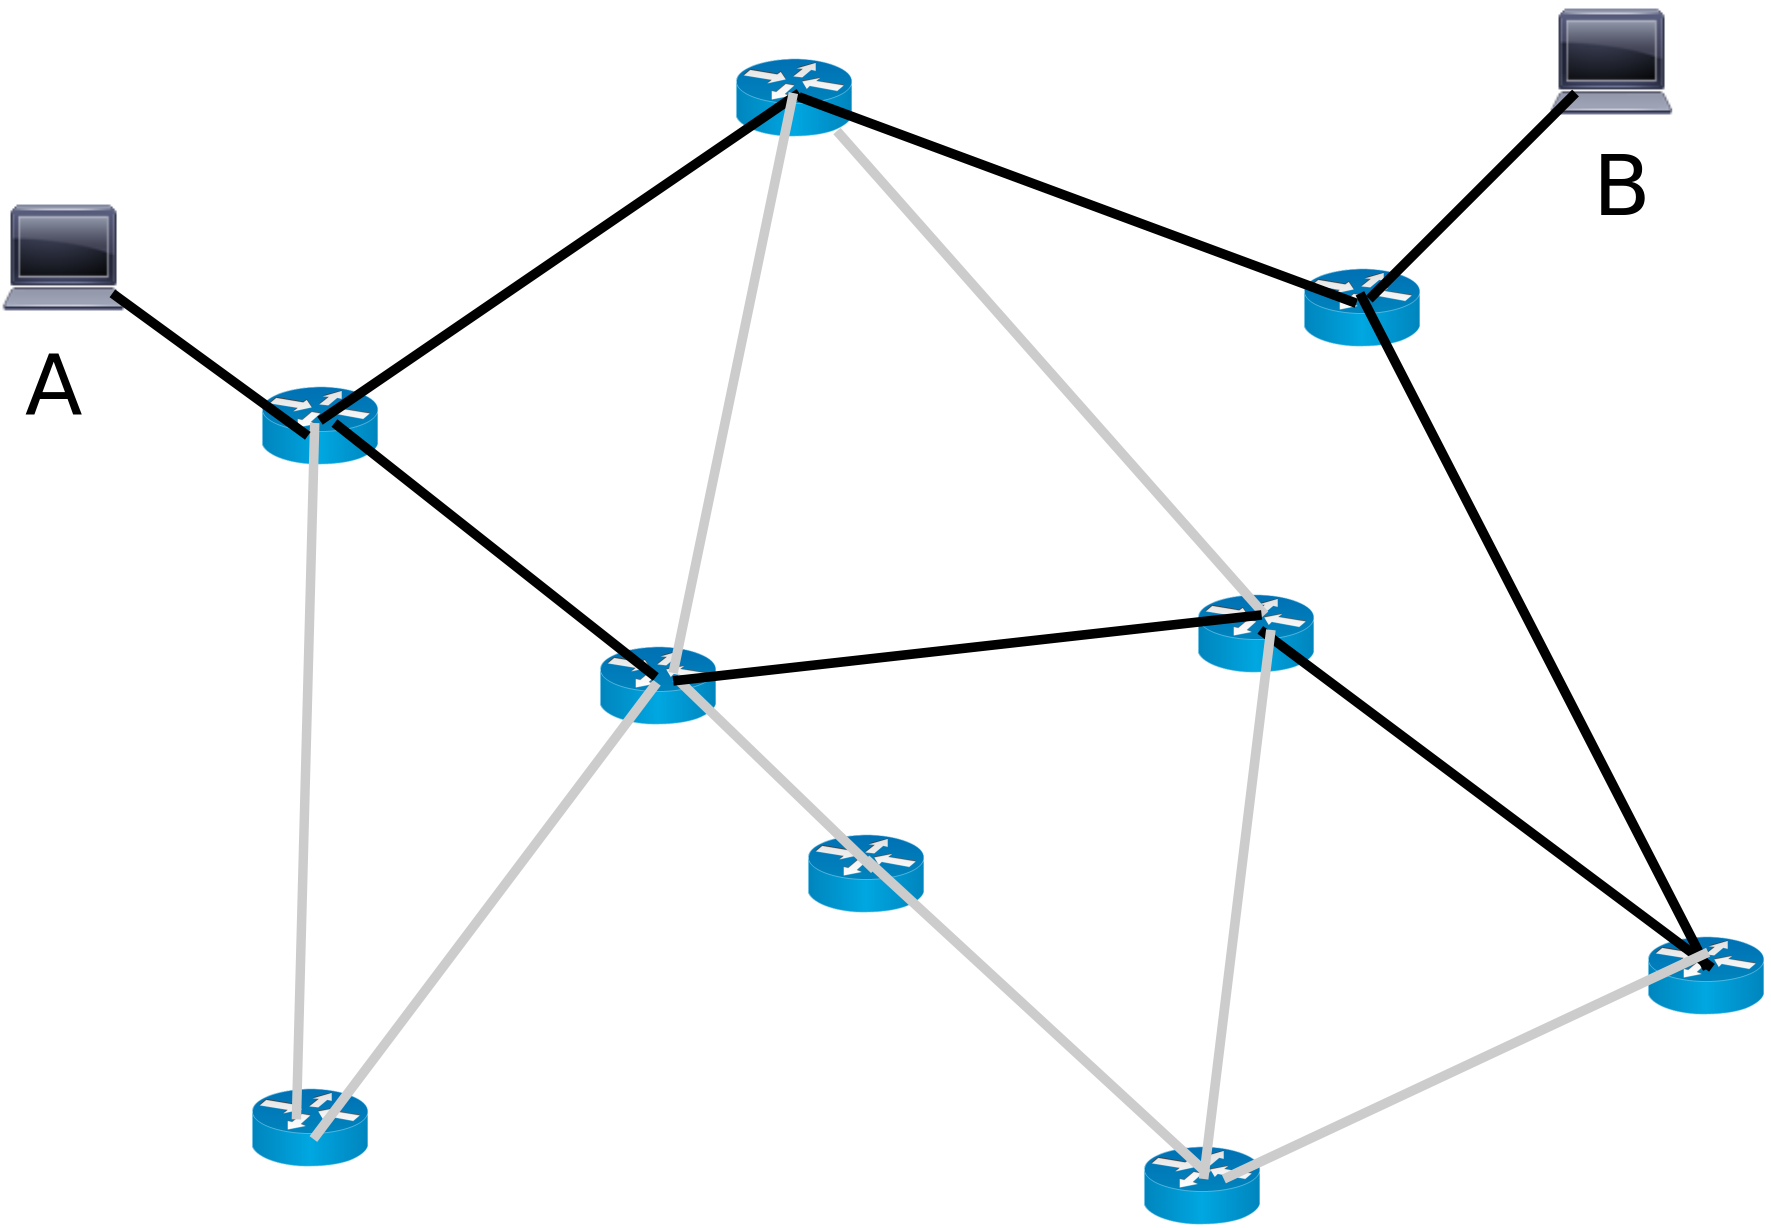
\includegraphics[width=.9\linewidth]{noisect.png}
     \caption{Множество маршрутов без пересечений}\label{Fig:Data4}
   \end{minipage}\hfill
\end{figure}

В качестве иллюстрации рассмотрим пример на рисунках \ref{Fig:Data3}, \ref{Fig:Data4}. Пусть все рёбра в этом примере имеют одинаковую пропускную способность. Тогда оба представленных варианта выбора маршрутов одинаковы по сумме длин входщих в него маршрутов, однако более предпочтительным для нас будет множество без пересечений (рис. \ref{Fig:Data4}), так как на общем для нескольких маршрутов канале может впоследствии образоваться узкое место; кроме того, такой набор маршрутов потеряет работоспособность в случае падения этого канала.\\
Задача же будет состоять в том, чтобы найти множество маршрутов заранее неизвестной мощности, и для каждого маршрута определить скорость передачи данных по нему. 
Найденное множество должно удовлетворять нескольким требованиям, а именно: \\
\begin{itemize}
\item Суммарная скорость передачи данных по всем маршрутам должна равняться требованию;
\item Найденное множество маршрутов должно иметь наименьшую стоимость среди всех множеств маршрутов
\end{itemize}

\newpage
\section{Формальная постановка задачи}
Дано:
\begin{itemize}
\item Граф $G(V, E)$ без кратных рёбер.
\item Отображение $bw: E \to \mathbb{R}_+$ --- остаточная пропускная способность каждого ребра графа в определённый момент времени, один и тот же для всех рёбер.
\item $s, d \in V$ --- вершина-источник и вершина-получатель
\item $r>0$ --- требование к пропускной способности 
\end{itemize}
\textbf{Введём некоторые дополнительные обозначения:}
\begin{itemize}

\item Обозначим как $P_i$ маршрут без циклов в $G$ --- чередующуюся последовательность вершин и рёбер графа $G$, каждые два соседних элемента которой инцидентны: $P_i = \{s, e^i_1, v^i_1, ..., v^i_{n-1}, e^i_n, d\}$, где $v^i_j \ne v^i_k, j \ne k$, $s, d \in E, e^i_j \in E, \forall j \in [1, n], v^i_k \in V, \forall k \in [1, n-1] $.

\item Пусть также $\mathbb{P} = \{P_i\}$ --- множество всех маршрутов из $s$ в $d$ в ненаправленном графе $G$, а $P \subseteq \mathbb{P}$ - некоторое его подмножество.

\item Назовём $mf:\ <G, s, d>\ \to \mathbb{R_+}$ --- величину максимального потока между вершинами $s$ в $d$ в графе $G$.

\item Пропускную способность отдельного маршрута обозначим $b:\ P_i \to \mathbb{R}$. Эта величина равна наименьшей из  остаточных пропускных способностей всех входящих в маршрут рёбер.

\item Каждому найденному маршруту будем ставить в соответствие его скорость $rate:\  P \to \mathbb{R_+^{|P|}}$, которая должна не превышать пропускной способности маршрута. 

\item Также введём функцию штрафа за пересечения между парой маршрутов $isect:\ P_i^2 \to \mathbb{R}_+,\ isect(P_i, P_j) = |\{e\ |\ e \in P_i \& e \in P_j, e \in E\}|*100$.

\item Стоимостью отдельно взятого маршрута будем считать $cost(P_i) = \frac{|P_i| - 1}{2*|V|} + \frac{mf(G, s, d) - mf(G \setminus P_i, s, d)}{b(P_i)}$ --- сумму двух величин: отношения длины маршрута к общему числу вершин в графе и отношения избыточной занимаемой пропускной способности к пропускной способности самого маршрута.

\item Стоимость множества маршрутов $cost(P) = \sum\limits_{P_i\in P} cost(P_i)\ + \sum\limits_{P_i, P_j \in P, \ i \ne j} isect(P_i, P_j)$ --- сумма стоимостей всех входящих в $P$ маршрутов и штраф за пересечения маршрутов этого множества между собой.

\item Будем называть множество маршрутов $P\in \mathbb{P}$ \textbf{допустимым}, если выполнены следующие условия:
\begin{itemize}
\item Суммарная скорость всех входящих в множество маршрутов равна заявленному требованию: $\sum\limits_{P_i\in P} rate(P_i) = r$.
\item Суммарная скорость всех проходящих через ребро графа маршрутов не превышает его пропускной способности: $\forall e \in E: \sum\limits_{P_i \ni e} rate(P_i) \le bw(e)$
\end{itemize}
\end{itemize}

\textit{\textbf{Необходимо найти}} допустимое множество маршрутов минимальной стоимости: $\argmin\limits_{P\in Q} cost(P)$, где $Q$ --- множество всех допустимых $P$.

\newpage
\section{Обзор существующих алгоритмов нахождения маршрутов для демультиплексированных соединений}
Уже существует множество алгоритмов поиска маршрутов на графе, решающих различные схожие с поставленной задачи, такие как поиск заранее заданного числа непересекающихся / имеющих минимальное количество пересечений / имеющих минимальную длину маршрутов. Цель нижеследующего обзора --- рассмотреть некоторые из алгоритмов решения похожих задач, определить их применимость или неприменимость к решению поставленной задачи и, возможно, выбрать один или несколько алгоритмов для того, чтобы на их основе построить алгоритм её решения.
\subsection{Критерии обзора}
\begin{itemize}
\item Входные данные алгоритма содержат заранее заданное \textit{количество маршрутов} $k$.\\ Заранее необходимое число маршрутов неизвестно, и его также необходимо определить, если алгоритм требует его в качестве входного параметра.
\item \textit{Оптимальность алгоритма.}\\ Под оптимальностью алгоритма будем понимать, что в случае, если существует хотя бы одно множество маршрутов, удовлетворяющее поставленной ранее задаче, то алгоритм находит решение поставленной задачи, которое имеет минимально возможную стоимость. В противном случае (если решения не существует или алгоритм не может его найти) алгоритм должен остановиться.
\item \textit{Временная сложность алгоритма.}\\ В сети могут происходить ситуации, когда одновременно необходимо обработать множество запросов, поэтому алгоритм должен быть способен обрабатывать их за короткое время; соответственно, временная сложность является важным фактором выбора того или иного алгоритма. 
\end{itemize}
\subsection{Рассмотренные алгоритмы}

\subsubsection{Жадный алгоритм}
Алгоритм работы:
\begin{enumerate}
\item В данном графе $G$ найти наилучший маршрут от $s$ к $d$ (например, с помощью алгоритма Дейкстры \cite{dijkstra}), поставим ему в соответствие скорость, равную его пропускной способности.
\item GOTO 1, если суммарная скорость найденных маршрутов не достила нужного значения, иначе работа окончена.
\end{enumerate}

Вышеизложенный алгоритм не является оптимальным в нашем понимании, то есть может не найти оптимальное решение, даже если оно существует и может быть найдено другими алгоритмами.
Ниже приведён пример случая, в котором выбор наилучшего в данный момент маршрута не оставляет достаточно свободных ресурсов для достижения требуемой скорости и требование уже не может быть достигнуто, в то время как при другом подходе решение может существовать.\\
Так, пусть в сети, показанной в примере на рис. \ref{Fig:greedy1}, крайний левый узел собирается передавать крайнему правому данные со скоростью 10 единиц. Очевидно, что при показанном выборе одного из маршрутов и отправке по нему данных с максимально возможной для него скоростью (6 единиц) требование будет уже недостижимо, хотя изначально была возможность выбрать 2 непересекающихся маршрута, удовлетворяющих требованию.

\begin{figure}[H]
   \begin{minipage}{0.5\textwidth}
     \centering
    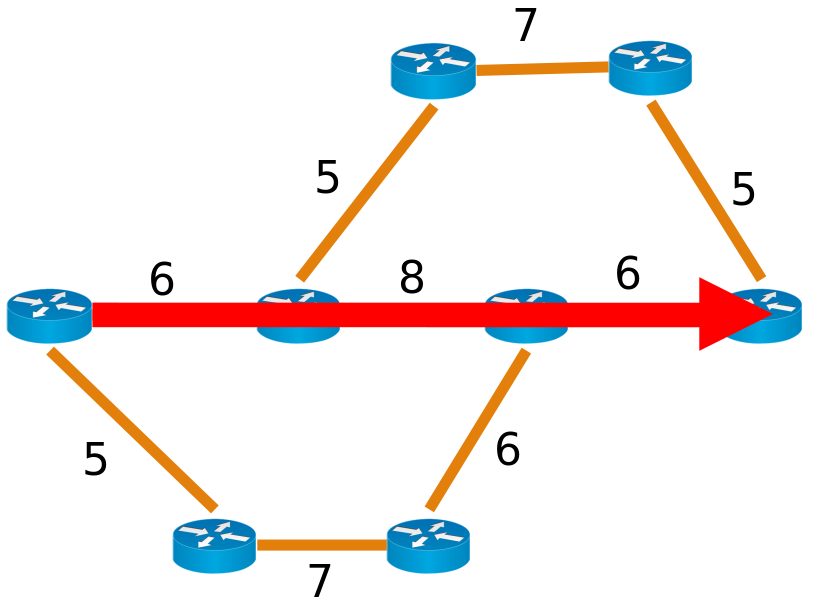
\includegraphics[width=.7\linewidth]{greedy1.png}
    \caption{Пример неудачного выбора маршрута\\ жадным алгоритмом}\label{Fig:greedy1}
   \end{minipage}
   \begin{minipage}{0.5\textwidth}
     \centering
     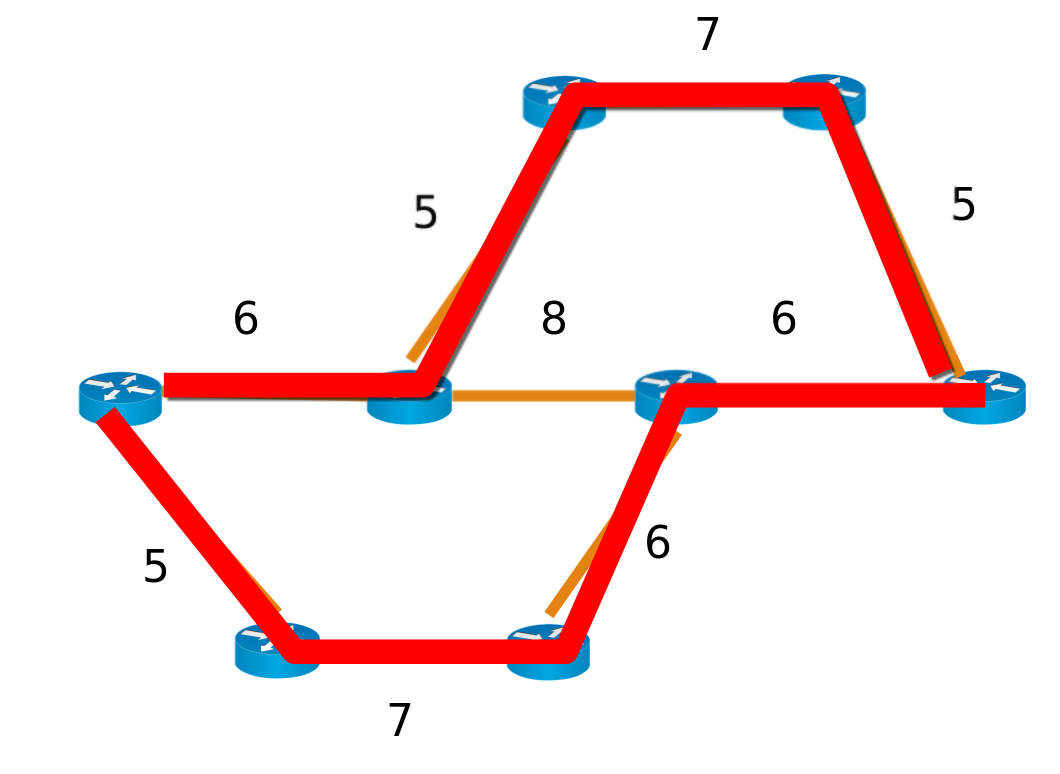
\includegraphics[width=.7\linewidth]{greedy2.png}
     \caption{Пример удовлетворяющего требованию\\ множества маршрутов}\label{Fig:greedy2}
   \end{minipage}\hfill
\end{figure}

Соответственно, хотя данный алгоритм и может быть применён к поставленной задаче, он не является оптимальным.

Сложность жадного алгоритма --- $O(k*|V|^2)$, где $k$ --- заданное число маршрутов.

\subsubsection{k-max-min disjoint paths}
Здесь рассмотрим не один конкретный алгоритм, а целое семейство алгоритмов, решающих задачу нахождения $k$ непересекающихся маршрутов между двумя точками. 
Вообще говоря, как показано в \cite{kmaxmin1}, эта задача относится к классу $NP$---трудных, что даёт полное право строить не точные, а эвристические алгоритмы её решения. 
Подробно алгоритмы данного семейства описаны в \cite{kmaxmin1, kmaxmin2, disjntNPC}, однако общая схема их работы следующая: сначала находится множество маршрутов от источника к получателю с помощью модифицированного алгоритма Дейкстры, после чего жадным алгоритмом выбирают k непересекающихся из них.

Данные алгоритмы находят $k$ \textit{непересекающихся} маршрутов, где $k$ должно быть задано, то есть они не решают проблему выбора необходимого количества маршрутов. Кроме того, может не существовать множества именно \textit{непересекающихся} маршрутов, удовлетворяющего заявленному требованию, хотя решение с пересекающимися маршрутами может существовать. Более того, на втором этапе работы алгоритма происходит "жадный"\  выбор, соответственно, возникает проблема, аналогичная проблеме предыдущего описанного алгоритма, а именно: алгоритм может не найти решение даже в случае, если оно существует.

Сложность алгоритмов этого семейства, описанных в \cite{kmaxmin1, kmaxmin2}, равна  $O(|E|*log|V| + V^2)$.

\subsubsection{Max Flow, или нахождение максимального потока}
Существует множество алгоритмов поиска максимального потока, такие как алгоритм Форда-Фалкерсона\cite{fordfson} или алгоритм проталкивания предпотока\cite{prepush}
Данные алгоритмы находят не множество маршрутов, а загрузку каждого канала, по которой позже можно составить множество маршрутов.\\ Достоинством этого подхода к решению является как то, что не нужно заранее знать количество используемых маршрутов, так и то, что он находит \textit{какое-то} множество маршрутов, удовлетворяющее требованию, если такое множество существует. Иначе говоря, решение (пусть и неоптимальное) будет найдено, если оно существует.\\
При этом данный алгоритм не накладывает на решение никаких штрафов за пересечения между маршрутами, кроме того, он решает задачу нахождения именно \textit{максимального} потока и при малом требовании может быть найдено плохое (то есть высокой стоимости) решение.

Таким образом, данный подход не годится для решения поставленной задачи, но, найдя величину максимального потока из точки в точку можно сразу проверить, не превышает ли её заявленное требование к пропускной способности. Более того, если требование не сильно отличается от найденной величины максимального потока, можно использовать этот подход для решения задачи.

Сложность алгоритма, решающего задачу о максимальном потоке, зависит от конкретного выбранного алгоритма. Так, например, для алгоритма Диница \cite{diniz} и алгоритма проталкивания предпотока \cite{prepush} она составляет $O(|V|^2*|E|)$, а для алгоритма Эдмондса-Карпа \cite{edmkarp} --- $O(|V|*|E|^2)$.

\subsection{MCMF, или Min-Cost Max-Flow}
MCMF\cite{stepsmel} сводит задачу к задаче поиска максимального потока минимальной стоимости, и начинает работу с изменения графа.

\begin{figure}[!htb]
   \begin{minipage}{0.5\textwidth}
     \centering
     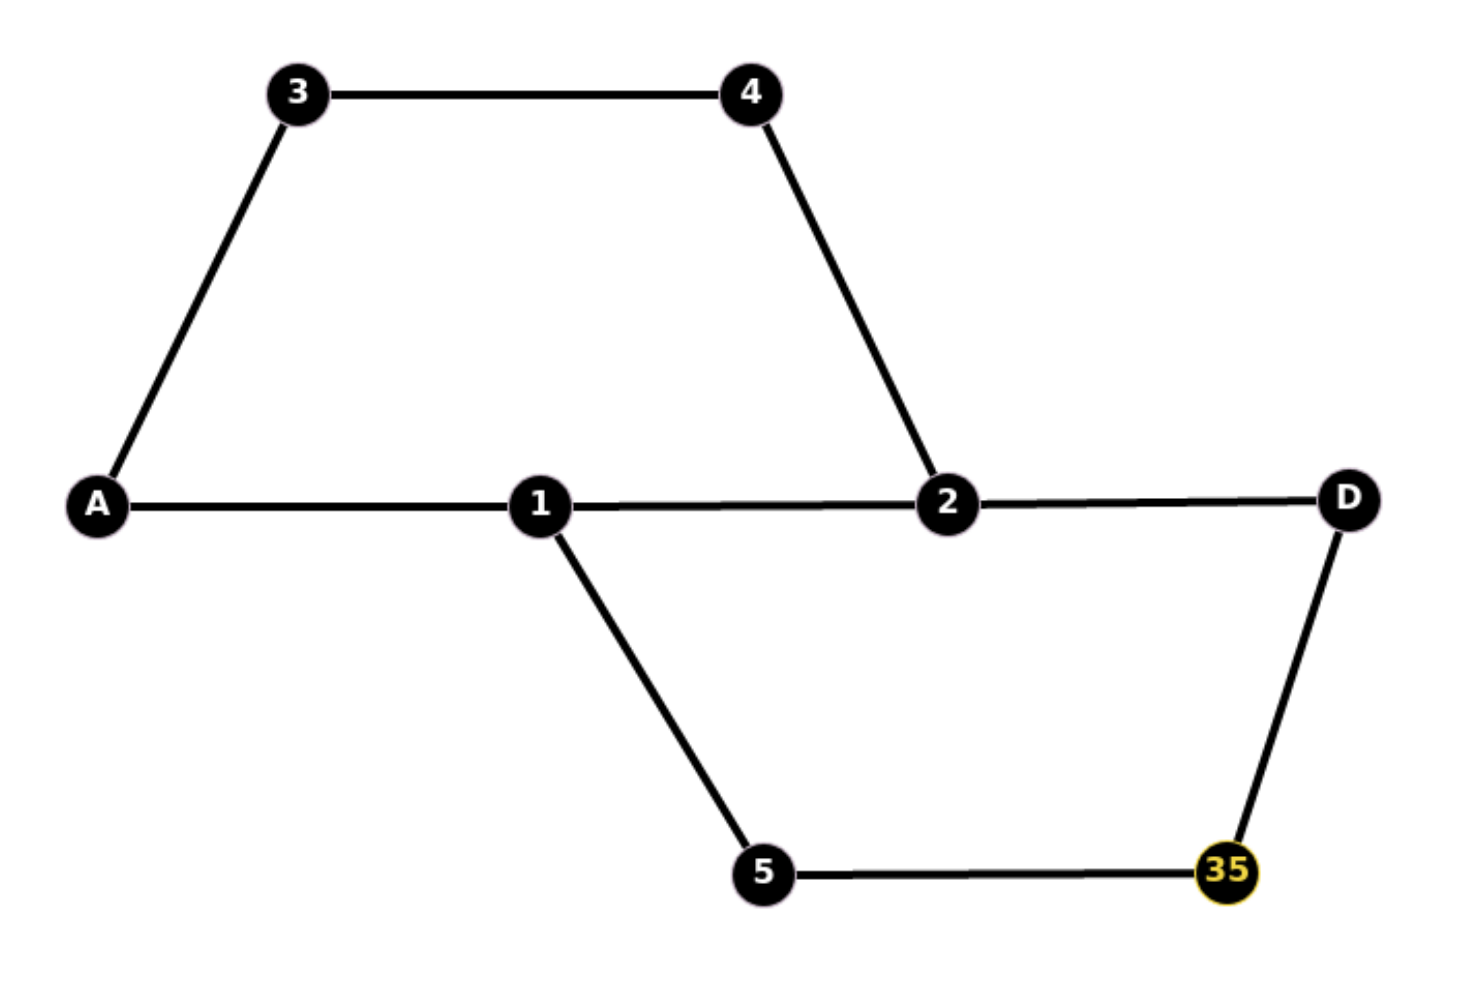
\includegraphics[width=.9\linewidth]{mc_bf.png}
     \caption{Исходный граф}\label{Fig:mc_bf}
   \end{minipage}
   \begin{minipage}{0.5\textwidth}
     \centering
     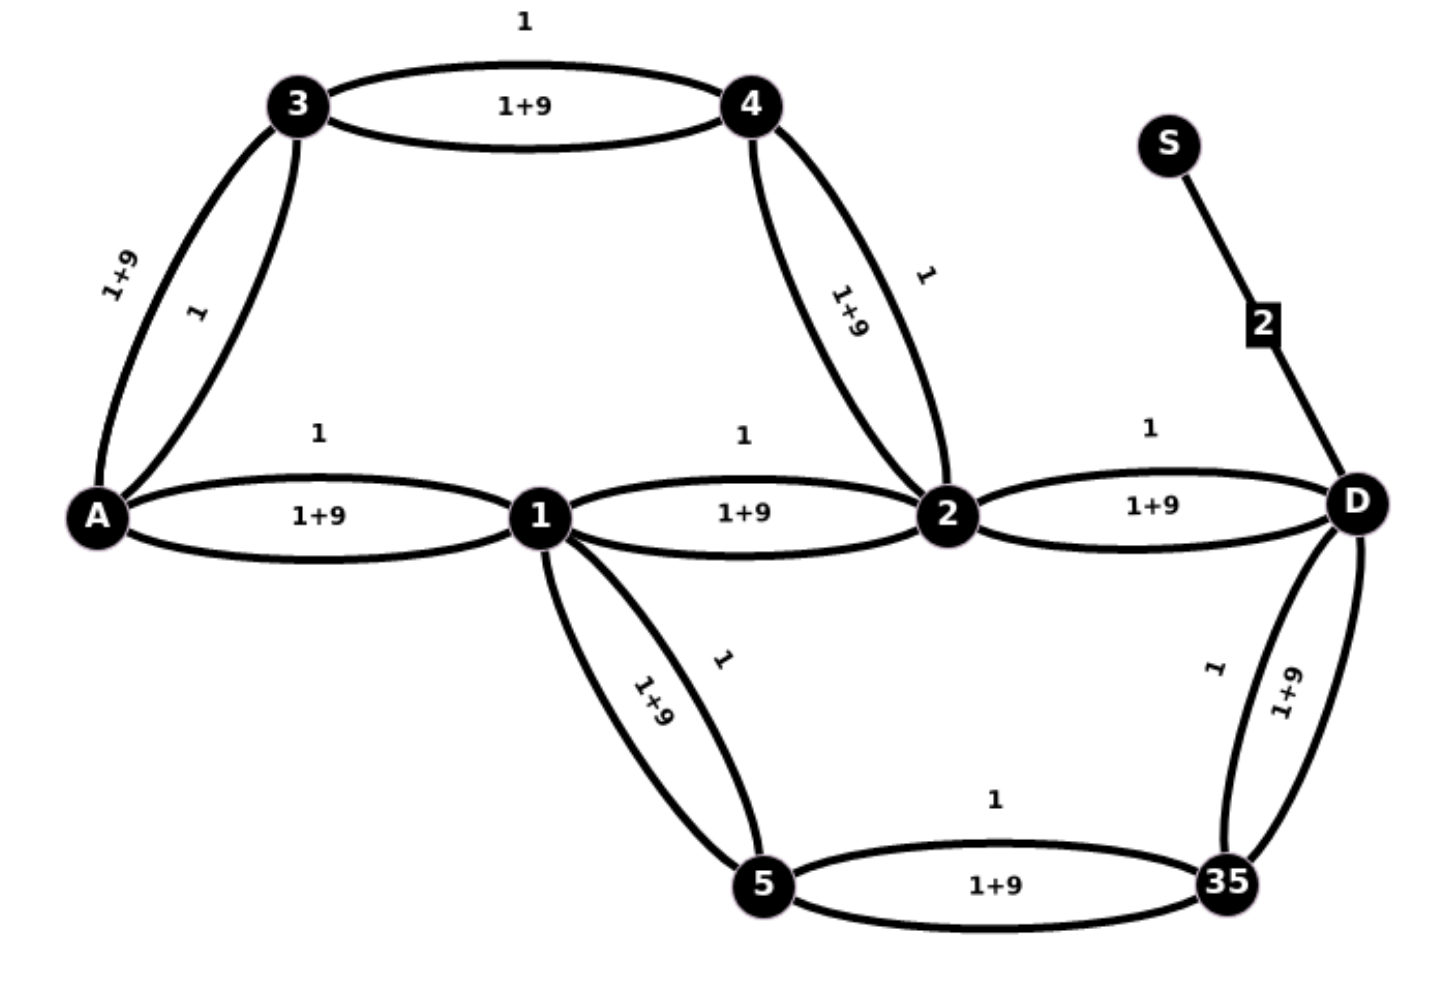
\includegraphics[width=.9\linewidth]{mc_af.png}
     \caption{Модифицированный граф}\label{Fig:mc_af}
   \end{minipage}\hfill
\end{figure}

Каждое ребро в графе заменяется на множество $k$ параллельных рёбер, где $k$ --- наперёд заданное требуемое количество маршрутов. Для каждого ребра из каждого такого множества установим стоимость, равную $1+i*|E|$, где $|E|$ --- количество рёбер в исходном графе, а $i$ --- порядковый номер ребра в своём множестве.
Для всех рёбер полученного таким образом графа их пропускная способность принимается равной единице. После этого добавляется узел-сток, который соединяется с узлом-получателем одним ребром единичной стоимости и пропускной способности $k$.\\
В примере на рисунках \ref{Fig:mc_bf} и \ref{Fig:mc_af} рассмотрен пример модификации графа для нахождения двух маршрутов между вершинами $A$ и $B$. Пропускная способность всех рёбер - единица, кроме ребра, соединяющего сток и вершину-получатель. Стоимость полученных рёбер указана рядом с ребром, пропускная способность указана на самом ребре,  соединяющем получателя со стоком.\\
Для полученного графа решается задача о нахождении максимального потока минимальной стоимости между вершиной-источником и добавленным стоком, после чего по потокам на каждом из рёбер восстанавливаются сами маршруты.
Таким образом, благодаря добавленному узлу-стоку число найденных маршрутов будет ограничено $k$, а за счёт высокой стоимости использования параллельных друг другу рёбер пересекающиеся по рёбрам маршруты будут выбраны в последнюю очередь.\\
Данный алгоритм обеспечивает нахождение $k$ маршрутов с минимальным пересечением, где $k$ ---наперёд заданное число, то есть не решается задача нахождения необходимого количества подпотоков. Кроме того, серьёзным недостатком данного алгоритма является то, что он не учитывает ни требование к скорости, ни пропускную способность каналов, и для решения поставленной задачи данный алгоритм в существующем виде неприменим.

Сложность алгоритма можно грубо оценить сложностью используемого алгоритма решения задачи о нахождении максимального потока $(maxflow)$.

\subsection{Выводы}
Как было установлено в результате обзора, ни один из рассмотренных алгоритмов не может быть применён к решению поставленной выше задачи. Однако, для дальнейшей модификации был выбран алгоритм MCMF. В частности, его преимуществом является то, что он не ограничивается только непересекающимися маршрутами, а лишь \textit{избегает} их. Ниже будет детально изложена как предлагаемая модификация MCMF, так и другие подходы к решению задачи.

\begin{table}[H]
\caption{Результат обзора}
\begin{center}
\begin{tabular}{|c|c|c|c|c|}
\hline
\ &  Жадный & k---max-min & Max Flow & MCMF \\
\hline
Находит число маршрутов & Да & Нет & Да & Нет \\
\hline
Оптимальное решение & Нет & Нет & Нет & Да \\
\hline
Сложность & $O(k*|V|^2)$ & $O(|E|*log|V| + V^2)$ & Зависит от конкретного алгоритма & (maxflow) \\
\hline
\end{tabular}
\end{center}
\end{table} 



\newpage
\section{Предложенные решения}
\subsection{Алгоритмы, требующие предварительных действий}
Так как введённая постановка задачи требует вычисления максимального потока для расчёта стоимости каждого маршрута, вполне уместно предложение заменить расчёт максимального потока в ходе работы алгоритма предварительными расчётами до начала работы основного алгоритма, по результатам которых уже во время работы можно будет получать решение, используя менее сложные алгоритмы. В настоящей работе рассматриваются две модели проведения этих подготовительных расчётов и, соответственно, два варианта алгоритма. 
Кроме того, выбор скоростей для набора маршрутов --- это отдельная задача, которая не рассматривается в рамках данной работы, поэтому в дальнейшем будем устанавливать скорость каждого маршрута либо равной его максимальной пропускной способности, либо разности между требованием и уже имеющейся суммарной пропускной способностью других выбранных маршрутов.

\subsubsection{Жадный с предрассчитанными маршрутами (PrecPths)} \label{pre_pth}
\paragraph{Подготовительные шаги}\mbox{}\\
$\forall s, d \in G: $
\begin{enumerate}
\item Найти множество всех маршрутов из $s$ в $d$
\item Для каждого маршрута найти стоимость в соответствии с постановкой задачи
\item Сохранить пару (маршрут, стоимость)
\end{enumerate}
В результате получается структура данных, в которой каждой паре точек на графе поставлено в соответствие множество пар маршрут-стоимость.

\paragraph{Основной алгоритм}\mbox{}\\
В результате работы алгоритма получается множество маршрутов, каждому из которых поставлена в соответствие скорость предачи данных по нему; и сумма скоростей всех маршрутов в этом множестве равна требованию к пропускной способности
\begin{enumerate}
\setcounter{enumi}{-1}
\item Изначально множество найденных маршрутов пусто
\item Выбрать из множества маршрутов между точками $s$, $d$ маршрут наименьшей стоимости.
\item Принять скорость маршрута равной меньшей из двух величин: пропускной способности маршрута или разности требуемой скорости и суммы скоростей всех уже имеющихся в множестве найденных маршрутов.
\item Добавить маршрут в множество найденных с рассчитанной скоростью. 
\item Увеличить стоимость всех ещё не выбранных маршрутов, имеющих пересечения с данным:
\begin{itemize}
\item Для каждого из ещё не выбранных маршрутов найти разность стоимости множества маршрутов и стоимости множества маршрутов при условии добавления этого маршрута в множество.
\end{itemize}
\item Если суммарная скорость всех найденных маршрутов равно требованию, работа алгоритма окончена. Иначе  GOTO 1. Если же по результатам очередной итерации суммарная скорость всех найденных маршрутов не изменилась, то считается, что решение не найдено и алгоритм возвращает пустое множество.
\end{enumerate}
\paragraph{Особенности подхода}\mbox{}\\
\begin{itemize}
\item[+] Нет необходимости искать маршруты алгоритма - маршруты уже посчитаны и нужно просто выбрать наиболее дешёвый
\item[-] В худшем случае, на каждом шаге придётся искать количество общих рёбер и пересчитывать стоимость $|V|!$ маршрутов (количество маршрутов между парой точек)
\end{itemize}

\subsubsection{Жадный с предрассчитанными весами (PrecWts)} \label{pre_wts}
\paragraph{Подготовительные шаги}\mbox{}\\
$\forall s, d \in G: $
\begin{enumerate}
\item Найти множество всех маршрутов из $s$ в $d$
\item Для каждого маршрута найти стоимость в соответствии с постановкой задачи
\item Добавить стоимость найденного маршрута к весу каждого ребра, через которое этот маршрут проходит
\end{enumerate}
В результате подготовительных шагов получаем вес каждого ребра в графе. Перед началом работы присвоим рёбрам графа соответствующие веса.

\paragraph{Основной алгоритм}\mbox{}\\
В результате работы алгоритма получается множество маршрутов, каждому из которых поставлена в соответствие скорость предачи данных по нему, сумма скоростей всех маршуртов в этом множестве равна требованию к пропускной способности.
\begin{enumerate}
\setcounter{enumi}{-1}
\item Изначально множество найденных маршрутов пусто
\item Найти маршрут наименьшей стоимости между точками $s$, $d$ (например, с помощью алгоритма Дейкстры) 
\item Принять скорость маршрута равной меньшей из двух величин: максимальной пропускной способности маршрута или разности требуемой скорости и суммы скоростей всех уже найденных маршрутов.
\item Добавить маршрут в множество найденных с рассчитанной скоростью. 
\item Увеличить вес всех рёбер, через которые проходит данный маршрут, на стоимость найденного маршрута.
\item Если суммарная скорость всех найденных маршрутов равно требованию, работа алгоритма окончена. Иначе  GOTO 1.
\end{enumerate}

\paragraph{Особенности подхода}\mbox{}\\
\begin{itemize}
\item[+] Найденных маршрутов как структуры данных не существует, после нахождения каждого маршрута необходимо увеличить всего не более $|E|$ рёбер на уже посчитанную величину
\item[-] На каждом шаге необходимо находить маршрут; например, алгоритмом Дейкстры, со сложностью $O(|V|^2)$
\end{itemize}

\subsubsection{Модифицированный MCMF (MCMF-mod)} \label{mcmfmod}
Предлагаемая модификация MCMF заключается в следующем:
\begin{itemize}
\item Вес каждого $i$-го добавляемого ребра будет приравниваться не $1+i*|E|$, как в оригинальном алгоритме, а $\frac{maxcap}{capacity} * (1+i*|E|)$, где $maxcap$ --- наибольшая из пропускных способностей рёбер графа, а $\frac{maxcap}{capacity}$  --- инвертированная пропускная способность ребра. Таким образом, маршрут с маленькой пропускной способностью будет выбран с меньшей вероятностью.
\item Так как при попытке восстановления маршрутов по результату работы алгоритма максимального потока может быть получен маршрут с одним или несколькими циклами, явно укажем, что циклы в маршруте удаляются.
\item Для выбора числа маршрутов $k$ была выбрана следующая простая стратегия. Изначально установим $k=1$, и запустим алгоритм поиска маршрутов.\\
После того, как было получено множество маршрутов, будем последовательно выбирать по одному самому дешёвому (согласно данного в постановке задачи определения) маршруту, задавать его скорость равной его же максимальной пропускной способности или разности требуемой скорости и сумме скоростей уже найденных маршрутов.\\
Итак, если требование с данным $k$ удовлетворено, то работа алгоритма останавливается, в противном случае увеличим $k$ на единицу и повторим ещё раз.
Здесь нужно отметить, что если алгоритм не может найти $k$ маршрутов, то некоторые маршруты в результате могут повторяться.
\item Дабы предотвратить вход в бесконечный цикл, установим правило, что если результаты работы на предыдущем и на текущем шагах не отличаются друг от друга, то алгоритм останавливается и возвращает пустое множество маршрутов, что свидетельствует об ошибке при поиске, так как больше, очевидно, уникальных маршрутов алгоритм не найдёт.
\end{itemize}

У данного алгоритма также имеются свои преимущества и недостатки перед другими вариантами:
\begin{itemize}
\item[+] Он не требует никаких подготовительных шагов, которые могут занимать продолжительное время, и не занимает пространство в памяти.
\item[+] В частности, он гораздо более подходит для работы с изменяющейся топологией, так как для некоторых (даже довольно небольших по количеству вершин и рёбер) топологий подготовительные шаги могут занимать несколько часов работы среднего по характеристикам компьютера (Intel Core i5-7200U, 2500 - 3100 MHz; 8 gb LPDDR3 RAM).
\item[-] На этапе поиска маршрутов стоимость никак не учитывается, а выбор производится из уже имеющихся маршрутов неизвестной стоимости, соответственно, найденной множество маршрутов может оказаться дорогим.
\item[+] Несмотря на это, пересечение найденных маршрутов всё ещё будет минимально. 
\end{itemize}


\newpage
\section{Экспериментальное исследование}
Целью экспериментального исследование было поставлено сравнение эффективности работы трёх предложенных алгоритмов, которая характеризуется следующими параметрами:
\begin{itemize}
\item Алгоритм \textit{\textbf{находит множество маршрутов}} и скорость передачи данных для каждого из них, удовлетворяющие поставленному требованию к пропускной способности, если существует хотя бы одно такое множество
\item \textit{\textbf{Стоимость}} найденного множества маршрутов
\end{itemize}

\subsection{Схема исследования}
Для проведения исследования были взяты топологии из TopologyZoo. Для каждой из них были случайным образом выбраны пропускные способности всех каналов в диапазоне $[300, 1000]$. Далее были выполнены подготовительные шаги для алгоритмов \textit{PrecPths} и \textit{PrecWts}. 

Отметим, что все алгоритмы исследуются на отдельном экземпляре топологии, независимо друг от друга, но на одном и том же наборе входных данных.

На каждой из рассматриваемых топологий многократно (в нашем случае - 1000 раз) выполняются следующие шаги:
\begin{itemize}
\item Случайным образом выбираются две точки, между которыми алгоритмы будут искать маршрут.
\item Найходится величина максимального потока $mf_i$ между этими вершинами в каждом из экземпляров топологии.
\item Выбирается наименьшая из них ($bound$), а в качестве требования фиксируется случайное число из диапазона $[\lfloor bound/2 \rfloor, bound)$. (Выбирается именно наименьшая величина для того, чтобы для всех алгоритмов на их топологиях априори существовало хотя бы одно допустимое множество маршрутов.)
\item Каждый алгоритм ищет множество, удовлетворяющее заданному требованию, на своём экземпляре топологии. Если множество не найдено, процент отказов данного алгоритма увеличивается. Если множество найдено, то находится и сохраняется его стоимость для дальнейшего анализа.
\end{itemize}

\subsection{Результаты исследования}

\begin{figure}[H]
     \centering
     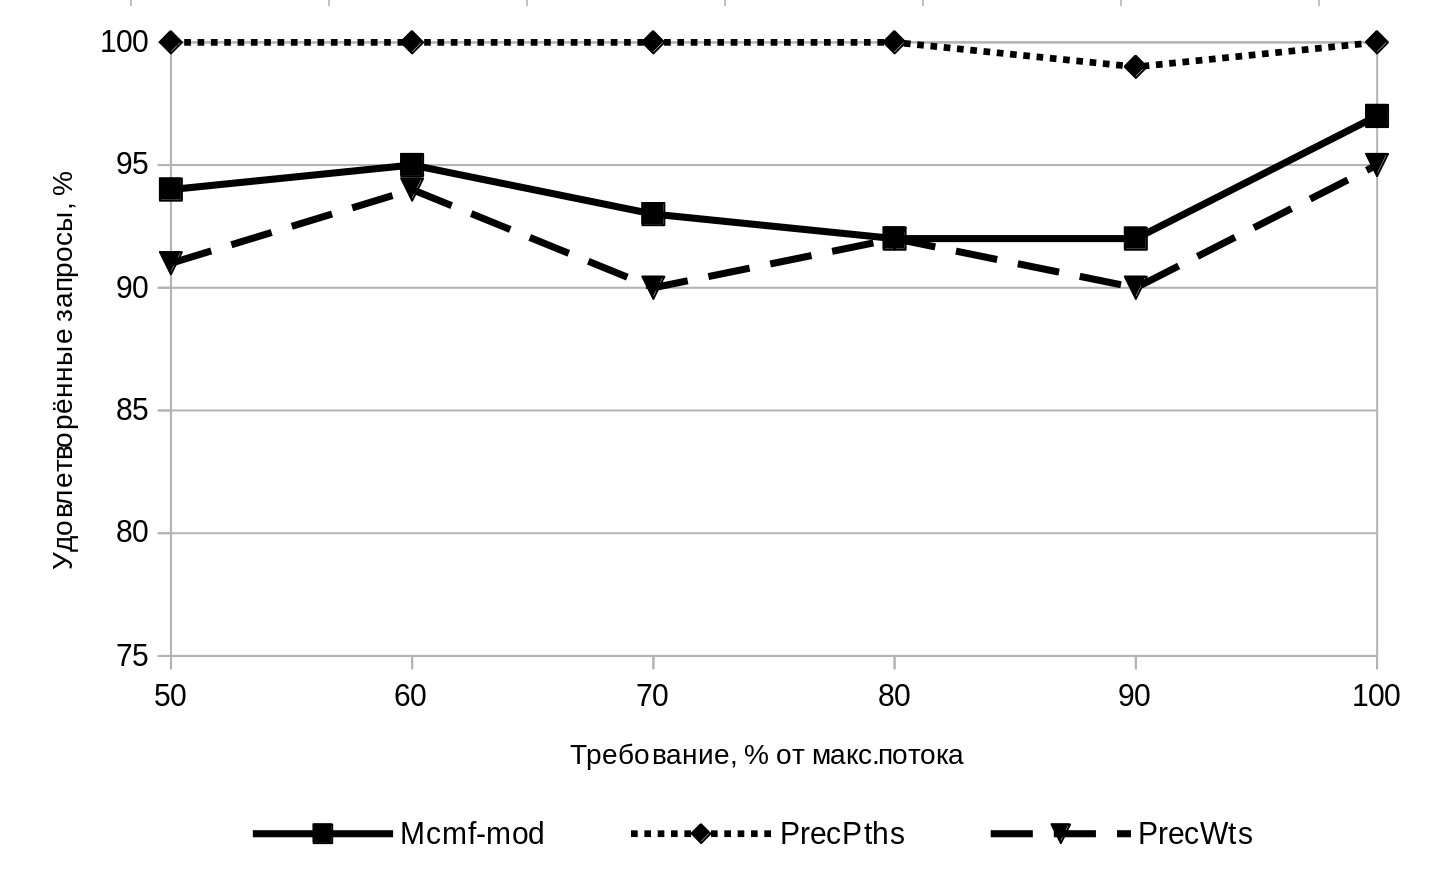
\includegraphics[width=.65\linewidth]{ch1.png}
     \caption{Процент удовлетворённых запросов в зависимости от требования к пропускной способности}\label{Fig:Chart5}
\end{figure}

\begin{figure}[H]
     \centering
     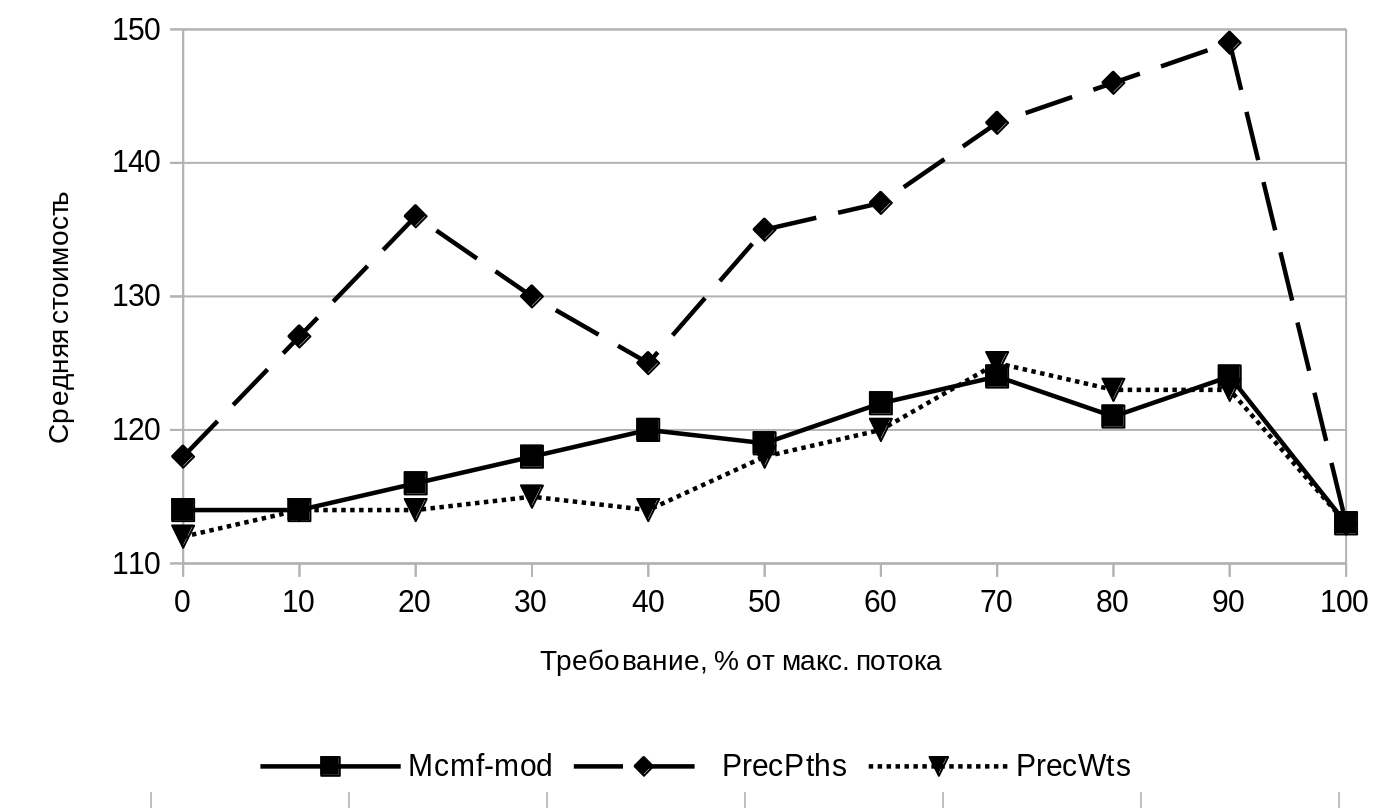
\includegraphics[width=.65\linewidth]{ch2.png}
     \caption{Средняя стоимость решения в зависимости от требования к пропускной способности}\label{Fig:Chart6}
\end{figure}

\begin{figure}[H]
     \centering
     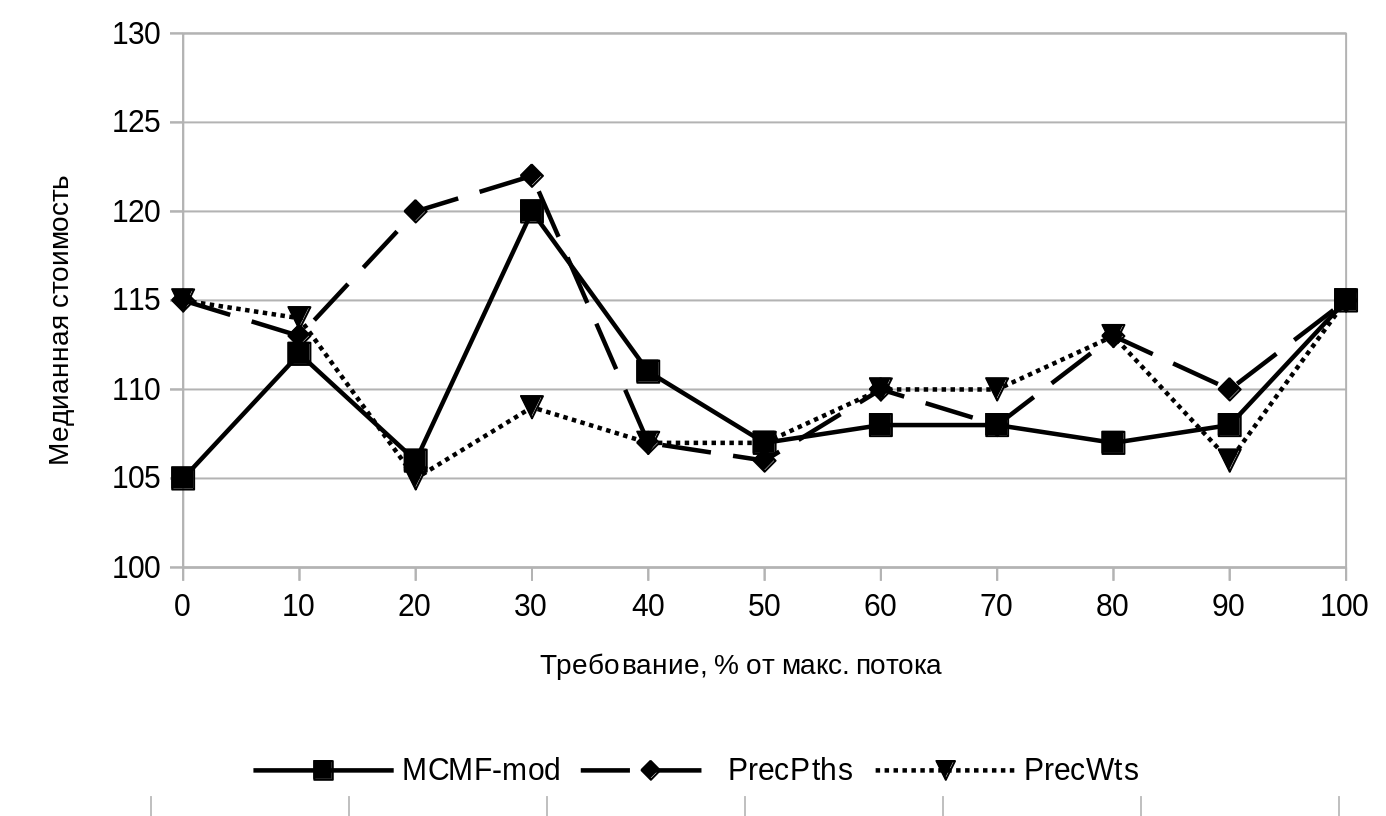
\includegraphics[width=.65\linewidth]{median.png}
     \caption{Медианная стоимость решения в зависимости от требования к пропускной способности}\label{Fig:Median}
\end{figure}



На рисунке \ref{Fig:Chart5} показан процент запросов, по результатам которых решение было найдено, в зависимости от требования к пропускной способности. На рисунке \ref{Fig:Chart6} показана усреднённая по рассмотренным топологиям стоимость найденного решения в зависимости от заявленного требования, а на рисунке \ref{Fig:Median} --- медианная стоимость.\\
Для более корректного обобщения данных (величины максимальной пропускной способности могут сильно отличаться), требование к пропускной способности на графиках показано в форме отношения требования к величине максимального потока между двумя точками.\\
Как видно из графика на рис. \ref{Fig:Chart5}, наилучшую точность имеет алгоритм \textit{PrecPths} --- он находит решение почти в 100\% случаев, тогда как \textit{PrecWts} и \textit{MCMF-mod} найдут решение в среднем в 87\% и 91\% случаев соответственно.\\
Однако, средняя стоимость найденных алгоритмом \textit{PrecPths} решений значительно превышает среднюю стоимость решений, полученных двумя другими алгоритмами, при этом медианная стоимость решений (рис. \ref{Fig:Median}), полученных тем же алгоритмом, менее отличается от результатов работы алгоритмов \textit{PrecWts} и \textit{MCMF-mod}. \\
Объясняется это тем, что алгоритм \textit{PrecPths} чаще других выдаёт в качестве решения множество маршрутов с аномально высокой стоимостью (что как раз объясняется тем, что часто в случаях, когда другие алгоритмы решение не находят, он находит решение, но оно имеет высокую стоимость), но в большинстве случаев их стоимость мало отличается от стоимости решений \textit{PrecWts} и \textit{MCMF-mod}.

\newpage
\section{Заключение}
В результате проведения данной работы были получены следующие результаты:
\begin{itemize}
\item Проведён обзор существующих алгоритмов нахождения маршрутов демультиплексированных соединений, по результатам которого был выбран алгоритм MCMF с целью его дальнейшей модификации для решения поставленной задачи.
\item Разработаны и реализованы три алгоритма поиска маршрутов демультиплексированных соединений, учитывающих текущее состояние сети.
\item Проведено экспериментальное исследование прототипов разработанных алгоритмов, которое показало, что алгоритм, описанный в \textit{\ref{mcmfmod}} имеет наибольший процент удовлетворённых запросов при одинаковой медианной стоимости получаемых решений.
\end{itemize}

В планы дальнейших исследований входит:
\begin{itemize}
\item Разработка алгоритма нахождения оптимальных скоростей для множества маршрутов, получаемого рассмотренными алгоритмами.
\item Более детальное исследование рассмотренных алгоритмов, в частности, сравнение результатов их работы с результатами работы переборных алгоритмов.
\item Разработка и реализация приложения контроллера ПКС для маршрутизации демультиплексированных соединений с использованием описанных алгоритмов.
\end{itemize}

\newpage
\begin{thebibliography}{14}
\bibitem{stepsmel}
E. Stepanov, R. Smelianski. On Analysis of Traffic Flow Demultiplexing Effectiveness

\bibitem{mpusage}
Q. D. Coninck and O. Bonaventure, "Tuning Multipath TCP for Interactive Applications on Smartphones," 2018 IFIP Networking Conference (IFIP Networking) and Workshops, Zurich, Switzerland, 2018, pp. 1-9, doi: 10.23919/IFIPNetworking.2018.8696520.

\bibitem{protos}
Habib, S., Qadir, J., Ali, A., Habib, D., Li, M., \& Sathiaseelan, A. (2016). The past, present, and future of transport-layer multipath. Journal of Network and Computer Applications, 75, 236–258.

\bibitem{mptcp}
RFC6824. TCP Extensions for Multipath Operation with Multiple Addresses. A. Ford, C. Raiciu, M. Handley, O. Bonaventure. January 2013.

\bibitem{sctp}
RFC4960. Stream Control Transmission Protocol. R. Stewart, Ed.. September 2007.

\bibitem{FDMP}
E. Chemeritskiy, E. Stepanov, R. Smelianski. Managing network resources with Flow (De) Multiplexing Protocol

\bibitem{dijkstra}
E. Dijkstra, “A note on two problems in connection with graphs,” Numerische mathematik, vol. 1, no.1, 1959, pp. 269-271

\bibitem{fordfson}
Ford L. R., Fulkerson D. R. «Maximal Flow through a Network», Canadian Journal of Mathematics. – 1956.

\bibitem{prepush}
Andrew V. Goldberg and Robert E. Tarjan. 1988. A new approach to the maximum-flow problem. J. ACM 35, 4 (Oct. 1988), 921–940.

\bibitem{diniz}
Dinitz, Yefim. (2006). Dinitz' algorithm: The original version and even's version. Lecture Notes in Computer Science. 3895. 218-240.

\bibitem{edmkarp}
Edmonds, Jack \& Karp, Richard. (2003). Theoretical Improvement in Algorithmic Efficiency for Network Flow Problems. Journal of the ACM. 19. 248-264.

\bibitem{kmaxmin1}
M. Doshi, A. Kamdar. Multi-Constraint QoS Disjoint Multipath Routing in SDN

\bibitem{kmaxmin2}
Jang-Ping S., Lee-Wei L., Jagadeesha R., Yeh-Cheng C. An efficient multipath routing algorithm for multipath TCP in SDN.

\bibitem{disjntNPC}
C-L Li, S. T. McCormic, and D. Simchi-Levi , " The Complexity of
Finding Two Disjoint Paths with Min-Max Objective Function ,"
Discrete Applied Mathematics, Vol. 26, No. 1, pp. 105-115, January
1990.
\end{thebibliography}


\end{document}
